%%%%%%%%%%%%%%%%%%%%%%%%%%%%%%%%%%%%%%%%%%%%%%%%%%%%%%%%%%%%%%%%%%%%%%
% LaTeX Template: Designer's CV
%
% Source: http://www.howtotex.com
% 
% Feel free to distribute this example, but please keep the referral
% to HowToTeX.com
% 
% Date: March 2012
%
% Modified by Lim Lian Tze to support multiple pages using fix provided at
% http://www.howtotex.com/templates/creating-a-designers-cv-in-latex/
% Date: November 2014
%%%%%%%%%%%%%%%%%%%%%%%%%%%%%%%%%%%%%%%%%%%%%%%%%%%%%%%%%%%%%%%%%%%%%%
% How to use writeLaTeX: 
%
% You edit the source code here on the left, and the preview on the
% right shows you the result within a few seconds.
%
% Bookmark this page and share the URL with your co-authors. They can
% edit at the same time!
%
% You can upload figures, bibliographies, custom classes and
% styles using the files menu.
%
% If you're new to LaTeX, the wikibook is a great place to start:
% http://en.wikibooks.org/wiki/LaTeX
%
%%%%%%%%%%%%%%%%%%%%%%%%%%%%%%%%%%%%%%%%%%%%%%%%%%%%%%%%%%%%%%%%%%%%%%

%%%%%%%%%%%%%%%%%%%%%%%%%%%%%%%%%%%%%
% Document properties and packages
%%%%%%%%%%%%%%%%%%%%%%%%%%%%%%%%%%%%%
\documentclass[a4paper,12pt,final]{memoir}

% misc
\renewcommand{\familydefault}{bch}	% font
\pagestyle{empty}					% no pagenumbering
\setlength{\parindent}{0pt}			% no paragraph indentation


% required packages (add your own)
\usepackage{polski}
\usepackage[utf8]{inputenc}
\usepackage{flowfram}										% column layout
\usepackage[top=1cm,left=1cm,right=1cm,bottom=1cm]{geometry}% margins
\usepackage{graphicx}										% figures
\usepackage{url}											% URLs
\usepackage[usenames,dvipsnames]{xcolor}					% color
\usepackage{multicol}										% columns env.
	\setlength{\multicolsep}{0pt}
\usepackage{paralist}										% compact lists
\usepackage{tikz}

%%%%%%%%%%%%%%%%%%%%%%%%%%%%%%%%%%%%%
% Create column layout
%%%%%%%%%%%%%%%%%%%%%%%%%%%%%%%%%%%%%
% define length commands
\setlength{\vcolumnsep}{\baselineskip}
\setlength{\columnsep}{\vcolumnsep}

% left frame
\newflowframe{0.2\textwidth}{\textheight}{0pt}{0pt}[left]
	\newlength{\LeftMainSep}
	\setlength{\LeftMainSep}{0.2\textwidth}
	\addtolength{\LeftMainSep}{1\columnsep}
 
% small static frame for the vertical line
\newstaticframe{1.5pt}{\textheight}{\LeftMainSep}{0pt}
 
% content of the static frame
\begin{staticcontents}{1}
\hfill
\tikz{%
	\draw[loosely dotted,color=ForestGreen,line width=1.5pt,yshift=0]
	(0,0) -- (0,\textheight);}%
\hfill\mbox{}
\end{staticcontents}
 
% right frame
\addtolength{\LeftMainSep}{1.5pt}
\addtolength{\LeftMainSep}{1\columnsep}
\newflowframe{0.7\textwidth}{\textheight}{\LeftMainSep}{0pt}[main01]


%%%%%%%%%%%%%%%%%%%%%%%%%%%%%%%%%%%%%
% define macros (for convience)
%%%%%%%%%%%%%%%%%%%%%%%%%%%%%%%%%%%%%
\newcommand{\Sep}{\vspace{1.5em}}
\newcommand{\SmallSep}{\vspace{0.5em}}

\newenvironment{Career Profile}
	{\ignorespaces\textbf{\color{ForestGreen} Career Profile}}
	{\Sep\ignorespacesafterend}
	
\newenvironment{Key experience}
	{\ignorespaces\textbf{\color{ForestGreen} Key experience}}
	{\Sep\ignorespacesafterend}
\newcommand{\CVSection}[1]
	{\Large\textbf{#1}\par
	\SmallSep\normalsize\normalfont}

\newcommand{\CVItem}[1]
	{\textbf{\color{ForestGreen} #1}}


%%%%%%%%%%%%%%%%%%%%%%%%%%%%%%%%%%%%%
% Begin document
%%%%%%%%%%%%%%%%%%%%%%%%%%%%%%%%%%%%%
\begin{document}

% Left frame
%%%%%%%%%%%%%%%%%%%%
%
% Upload your own photo using the files menu
\begin{figure}
	\hfill
	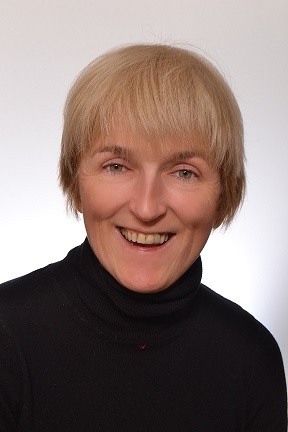
\includegraphics[width=1\columnwidth]{zeby.jpg}
	\vspace{-7cm}
\end{figure}

\begin{flushright}
	\small
	\color{White}....................................\\
	\Sep
	\color{Black}
	Beata Greń-Onderko \\
	\url{beongren@gmail.com}  \\
	(+44) 7448 245462\\
	d.o.b.: 31st August 1963\\
	Polish full driving license\\
	CRB on demand
\end{flushright}\normalsize
\framebreak


% Right frame
%%%%%%%%%%%%%%%%%%%%
\Huge\bfseries {\color{ForestGreen} Beata Greń-Onderko} \\
\Large\bfseries  Health care assisant \\

\normalsize\normalfont

% Career Profile
\begin{Career Profile} 
I am a committed, hard working person who wants to make use of her abilites to listen to people, understand their needs, patiently take care and respect them. 
I have livelong experience in childcare (in Poland, France and UK) but I am willing to learn and participate in professional training for health care assistant, as I have experience in this kind of care.
I am full of energy, punctual and open to new challenges.
\end{Career Profile}

%Key experience
\begin{Key experience}
During the last summer holiday, I took care of elderly woman, 83 years old. I worked for her voluntarily for two months (after that I had to move to UK). She is completely blind and struggles with diabetes. I helped her almost every day with shopping, household duties and  I listened with great pleasure to her life stories or poems she loves to recite. This experience showed me that taking care of elderly people is both for me and for them pleasant, and that it's the job I am called for. 
\end{Key experience}

% Work experience
\CVSection{Work experience}

\CVItem{20th October 2016- ...}\\
Weekend Cook in Westbank Care Home \\
\begin{itemize}
\item{Cooking for more than 40 residents}
\item{Preparing breakfast, lunch, dinner, desserts, birthday cakes}
\item{Works alone or with a help of the kitchen assistant}
\item{Approximately 24 hours per week}
\end{itemize}
\CVItem{September 2015-…}\\
Au pair for two children : girl 22 months, girl 4.5 years old in Ross-on-Wye, UK
\SmallSep

\CVItem{October 1986-June 1987}\\
Afternoon babysitting in family orphanage: girl( 8 years old); boy (8 years old);girl aged 12 with schizophrenia;
\SmallSep

\CVItem{1988-89}\\
24h/7 babysitting of 9-month old baby girl; 
\SmallSep

\CVItem{July 1990-August 1991}\\
Au pair in Ventabren, France; 2 children: boy aged 1,5 and boy aged 3 as well as taking care of the house (cleaning, cooking, laundry etc.)
\SmallSep

%Training and Courses 
\CVSection{Training and Courses}
\CVItem{ 03rd October 1985 -19th May 1986}\\
\underline{First aid course} at Polish Red Cross at PRC Wrocław
\SmallSep

\CVItem{August 1986}\\
One month \underline{language scholarship} founded by French Embassy at University of Grenoble, France
\SmallSep

\CVItem{02nd March 2009-30th June 2009	}\\
Training in Social Integration Center (Centrum Integracji Społecznej) in 	Wrocław. Aim: schooling in \underline{licensing and running social cooperative (446 hours)}
\SmallSep

\CVItem{10th September 2009-19th December 2009}\\
\underline{English language course} at Pre-Intermediate level in Yellow Language Center 	Sp. z.o.o  (64 hours)
\SmallSep
\clearpage
\framebreak
\framebreak
\CVItem{January -August 2010 }\\
Participation in „Women professionally active- It's me” project concerning: 60h of \underline{UE projects management} training, 8h of \underline{labour legislation} training, 30h of \underline{computer skills} training (MS Office), 8h of \underline{labour market} training, 8h of \underline{psychology} workshop, 8h \underline{auto presentation} skills training,  \underline{english language course} finished with TOEIC exam
\SmallSep

\CVItem{2009-2011}\\
\underline{French language course} at level B2/C1 in Alliance Francais Language School in Wrocław (3 semesters)
\SmallSep

\CVItem{October 2014-July 2015}\\
\underline{English language course} at A2 level (coursebook A2/B1)
with final exam
\SmallSep

% Education
\CVSection{Education}
\CVItem{1982-1987}\\
Studies at Faculty of National Economics at Oskar Lange's Academy of Economics (now University of Economics) in Wrocław
\SmallSep


% Skills
\CVSection{Skills and Interests}
\CVItem{Languages}
\begin{multicols}{3}
\begin{compactitem}[\color{ForestGreen}$\circ$]
	\item English A2
	\item French  B2
	\item German  A1
\end{compactitem}
\end{multicols}
\SmallSep

\CVItem{Interests}
\begin{multicols}{3}
\begin{compactitem}[\color{ForestGreen}$\circ$]
	\item Natural medicine and herbalism
	\item Gardening
	\item Sports: fitness and skiing 
	\item Classical music 
	\item Films and  festivals
\end{compactitem}
\end{multicols}
\Sep 

% References
\CVSection{References}
References upon request.

%%%%%%%%%%%%%%%%%%%%%%%%%%%%%%%%%%%%%
% End document
%%%%%%%%%%%%%%%%%%%%%%%%%%%%%%%%%%%%%
\end{document}